% Generated by thesis/ch7/exp2/networks.py -- do not edit by hand.
\begin{sidewaysfigure}
  \centering
  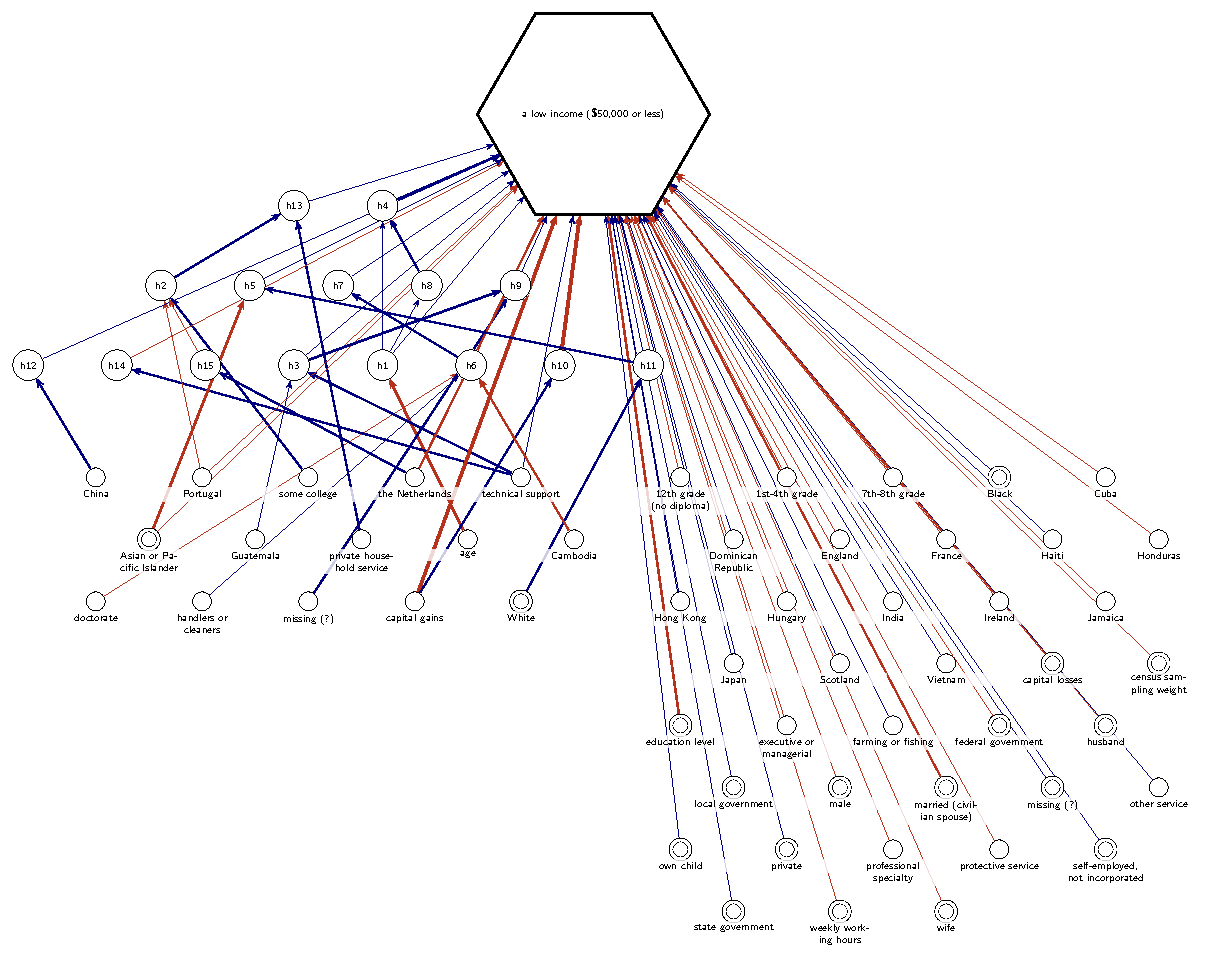
\includegraphics[width=\textheight,height=0.78\textwidth,keepaspectratio]{figures/exp2/networks/adult-s6-raw}
  \caption{Adult, seed 6 (adult-s6): the network as trained, before any explanation, in full. Inputs at the bottom (every input column its own node), hidden units by depth, the output at the top; 53 of 107 input columns are connected, with 15 hidden units and 77 enabled connections. Blue: positive weight (raises the score); red: negative weight (lowers it); thicker: larger weight. Orange outline and up arrow: raises the final prediction; teal and down arrow: lowers it; grey and double arrow: depends. Not used (no connection; 54 columns): never worked, self-employed, incorporated, without pay, 10th grade, 11th grade, high-school graduate, master's degree, preschool, professional school degree, 5th-6th grade, 9th grade, associate degree (academic), associate degree (vocational), bachelor's degree, divorced, married to a member of the armed forces, married, spouse absent, never married, separated, widowed, missing (?), administrative or clerical, sales, transport or moving, armed forces, craft or repair, machine operator or inspector, not in a family, other relative, unmarried, American Indian or Eskimo, other race, Germany, Greece, Canada, Iran, Italy, Laos, Mexico, Nicaragua, outlying US territories (Guam, US Virgin Islands), Peru, the Philippines, Poland, Puerto Rico, 'South' (as recorded), Taiwan, Thailand, Trinidad and Tobago, the United States, Colombia, Yugoslavia, Ecuador and El Salvador.}
  \label{fig:exp2-net-adult-s6-raw}
\end{sidewaysfigure}
